%\documentclass[aps,preprint,amsmath,amssymb]{revtex4-1}% APS journal style
%\documentclass[aps,reprint,amsmath,amssymb,prl]{revtex4-1}% APS journal style prl physical review letters
\documentclass[aps,reprint,amsmath,amssymb,pra]{revtex4-1}% APS journal pra default
%\documentclass[aps,reprint,amsmath,amssymb,prl,longbibliography]{revtex4-1}% to show the title of the articles in the bibliography
\usepackage{graphicx}% Include figure files
\usepackage{dcolumn}% Align table columns on decimal point
\usepackage{bm}% bold math
\usepackage{hyperref}% add hypertext capabilities
%\usepackage{lineno}
%\linenumbers
%\bibliography{natbib}

\begin{document}
\title{A toy model to understand the dynamics of the vortical motions in turbulent boundary layers}
\author{J.C. Cuevas Bautista}
\email{jcc1@wildcats.unh.edu}
\affiliation{University of New Hampshire, Department of Mechanical Engineering, Durham 03824, USA.}
\date{\today}
\begin{abstract}
\noindent 
Recent studies indicate that the structure of the turbulent boundary layer at high Reynolds number (\textit{Re}) is composed of large uniform momentum zones segregated by fissures of concentrated vorticity. Experiments reveal that the dimensionless fissures thickness (scaled by boundary layer thickness) is $\mathcal{O}(1/\sqrt{Re})$ and the dimensionless streamwise velocity jump across a fissure scales with the friction velocity $\mathcal{O}(u_{\tau})$. A toy model that captures the essential elements of the turbulent boundary layer structure at high \textit{Re} is constructed to evaluate the long-time averaged flow statistics of the boundary layer. First, a ``master'' instantaneous  streamwise velocity profile in the wall-normal direction is constructed by placing a discrete number of fissuress across the boundary layer thickness. The number of fissures and their wall-normal locations follow scalings informed by the Mean Momentum Balance (MMB) theory. Next, the wall-normal positions of the fissures are allowed to randomly move in the wall-normal direction creating a statistically independent second instantaneous velocity profile. This process is then repeated to create an ensemble of instantaneous velocity profiles from which average statistics of the turbulent boundary layer can be computed and assessed. The statistics of the toy model are compared to statistics acquired in turbulent boundary layers at high \textit{Re}.
\end{abstract}
\keywords{turbulent boundary layer, uniform momentum zones, vortical fissures and Mean Momentum Balance theory.}
\maketitle
\section{\label{sec:intro} Introduction}
Turbulent boundary layers and their mechanism are one the most active research areas in fluid mechanics~\citep{kline1967,head1981,heist2000}. Due to their chaotic behaviour, deterministic approaches are not possible. Thus there is a general consensus in the scientific community that turbulent boundary layers exhibit similar statistical properties, hence most studies relies in the reproducible averaging techniques.  As a consequence, part of the flow history is lost in this approach. A recent idea attempts to explain the particular shape of the mean streamwise velocity profile as the product of the long-time average of multiple instantaneous velocity profiles with different uniform momentum zones (UMZs)~\citep{mca1995,umz2015}. The coordinates convention for the mean flow are positive in the $x$ direction (streamwise), positive in the $y$ direction (wall normal) and  positive in the $z$ direction (spanwise). 

Adrian \textit{et al}.~\cite{mca1995} made two important observations about the structure of turbulent boundary layers. First observation indicates that zones of remarkable constant streamwise momentum exist throughout the boundary layer. Second that these regions seem to be bounded by thin viscous-inertial shear layers.  They also indicated that these structural properties are exclusive of the instantaneous velocity profiles which contribute to the mean statistical properties. Furthermore  Charitha \textit{et al}.~\cite{umz2015}
have studied the presence of UMZ in turbulent boundary layers by compare particle image velocimetry (PIV) data sets with generated synthetic instantaneous velocity fields. The established criteria to detect UMZs was compute the probability density function (p.d.f.) of random instantaneous PIV velocity profiles. Then the UMZs are associated with the locals maxima (modal velocity) in the p.d.f., the number of UMZs are determined by the modal velocities. The same analysis was applied to the synthetic velocity fields which also evidenced different modal velocities in the instantaneous p.d.fs. We remark unlike of~\cite{umz2015} in our toy model the existence of UMZs is already assumed and it pretends to explain how they are distributed and affect the mean streamwise statistics in the turbulent boundary layer. \\
In contrast with the traditional statistical approach, constructing the mean velocity profile by superposition of instantaneous velocity profiles with a different UMZs distribution allow us to examine in detail the individual history of the flow and explain the layers structure of turbulent flows.
The phenomenological and experimental description of the structure and origin of the uniform momentum zones through boundary layer has been studied by several authors~\citep{mca1995,amt2000,umz2015}. They suggest that UMZ are the result of the interaction of a wider range of structures that populate the turbulent boundary layer\cite{amt2000} such as hairpins and streamwise vortices. Adrian \textit{et al}.~\cite{amt2000} have made a thoroughly  study about how the vortex structures are organized and segregate the UMZs in turbulent boundary layers. An important conceptual scenario noted by ~\cite{amt2000} states that packets of vortex structures aligns in the streamwise direction creating a net effect of zones with a quasi-uniform momentum. Vortex structures are also referred as vortical fissures or vortex tubes when they represent the transversal section of a hairpin vortex in the streamwise-wall normal plane~\cite{amt2000}.  
Priyadarshana \textit{et al}.~\citep{priya2007} makes a good representation of the vortical fissures and their distribution in the instantaneous streamwise velocity profile (see Fig.~\ref{fig:vortical_fissures}). 
\begin{figure}[b]
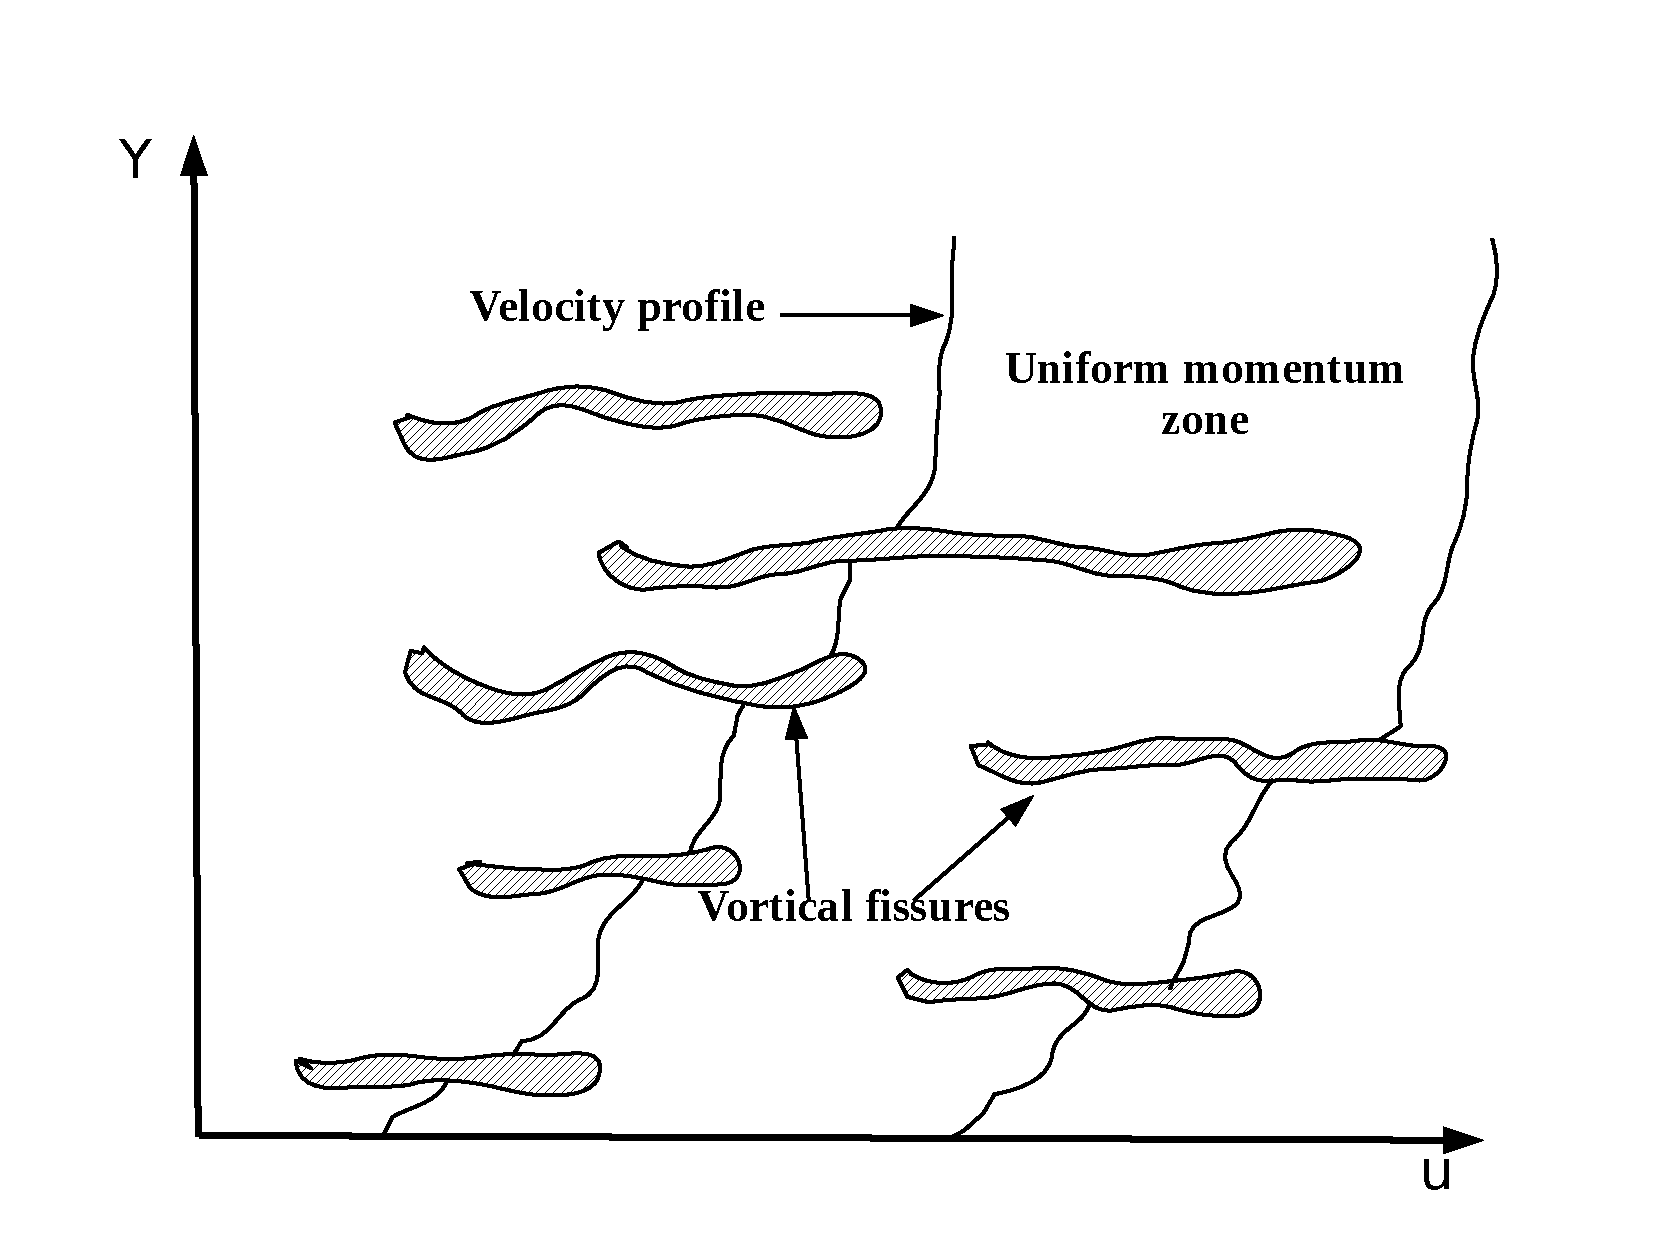
\includegraphics[scale=0.305]{figures/uniform_velocity_vortical_fissures}
\caption{\label{fig:vortical_fissures} Pictorial representation of instantaneous velocity profiles like zones of uniform momentum separated by zones of concentrated vorticity (vortical fissures). Where $U$ is the mean velocity in the x direction (streamwise) and $y$ is the wall normal coordinate.
Adapted from~\citep{priya2007}}
\end{figure} 
Vortical fissures are zones of concentrated vorticity that can
be spread by turbulent advection to regions where the mean viscous force is negligible. It has been shown using dimensional
analysis and scaling arguments that the thickness of the vortical fissures scales with the Reynolds as $\mathcal{O}(1/\sqrt{Re})$~\citep{tennekes1968}, thus as $Re$ increases, the thickness of the vortical fissures decreases. In the toy model presented here the thickness of vortical fissures is assumed negligible.

The zonal arrangement represented in Fig.~\ref{fig:vortical_fissures} could give us an insight to the traditional structure of layers in the mean velocity profile. In the proposed model here, this is explored by using different statistical distribution for perturbing the wall normal position of the vortical fissures (see Sec.~\ref{sec:nm}). 
Some models have achieved  notable results in reproduce the dynamics and the statistical properties of turbulent boundary layers by using different structures as hairpin structures~\citep{adrian2007} or eddy structures~\citep{perry1995}. However these models depend directly in the attached eddy hypothesis where the geometry of the eddies arising from the wall must be known in order to reproduce correctly the wall and the wake structure of the boundary layer. The model employed herein does not depend on specific geometries, instead it is based in the existence of two structure motions, UMZs and vortical fissures. These later are allowed to move randomly through the boundary layer following a scaling for the inertial region derived from MMB theory (see Sec~\ref{subsec:toymodel}). The   analysis of this scaling would help to explain the boundaries and the physical properties of the mean structure of the turbulent boundary layers (see Sec~\ref{subsec:4ls}). 
In this paper we present a simplified toy model to reproduce the higher order moments of the streamwise turbulent boundary layers. The numerical model can be tweaked in such way that we can verify if the long-time average of the instantaneous uniform-momentum zonal structures reproduces reasonably the physical and statistical properties of turbulent wall-bounded flows. Regarding this, different boundary conditions are explored in the layers I, II and III of the four-layer structure (see Sec~\ref{subsec:4ls}). DNS data for a channel flow at friction Reynolds number $\delta^+=\delta u_{\tau}/\nu\approx 5200$~\cite{leemoser2015} (where $u_{\tau}=\sqrt{\tau_{\omega}/\rho}$ is the friction velocity, $\tau_{\omega}$ is the mean wall shear stress, $\nu$ is the kinematic viscosity and $\delta$ is the boundary layer thickness) along with scaling reported by MMB theory was used to build the model. 

\section{\label{sec:nm} Numerical Methods}
\subsection{Four-layer structure\label{subsec:4ls}}
The traditional hierarchy of layers in turbulent boundary layers, i.e. the viscous sublayer, buffer layer, logarithmic layer and the outer layer is described extensively in standard textbooks on turbulence \cite{tenelumley,pa,mathieu}. However we will provide a briefly discussion about the layers structure based in the alternative approach of the MMB theory~\citep{wei2005,fife2005}. Klewicki \textit{et al.}~\citep{Klewickimmb} also describes in detail how the MMB theory predicts the physical and scaling behaviours of the so called four-layer structure in wall bounded-flows in analogy with the classical theory.  The velocity and  length scales of the emergent four-layer structure in the mean streamwise velocity profile are summarized in Table~\ref{tab:4layerstructure}.

\begin{table}[htb]%
\caption{\label{tab:4layerstructure}%
Scaling associated to the four layer structure from MMB theory. $\Delta y$ represents the thickness of the layer while $\Delta u$ is the velocity increment associated to that layer in the turbulent boundary layer~\citep{Klewickimmb}.
}
\begin{ruledtabular}
\begin{tabular}{ccc}
\textrm{Layer}&
\textrm{$\Delta y$}&
\textrm{$\Delta u$}\\
\colrule
I &$\mathcal{O}(\nu/u_{\tau})(\lesssim 3)$&$\mathcal{O}(u_{\tau})(\lesssim 3)$\\
II &$\mathcal{O}(\sqrt{\nu\delta/u_{\tau}})(\simeq 1.6)$&$\mathcal{O}(U_{\infty})(\simeq 0.5)$\\
III &$\mathcal{O}(\sqrt{\nu\delta/u_{\tau}})(\simeq 1.0)$&$\mathcal{O}(u_{\tau})(\simeq 1)$\\
IV &$\mathcal{O}(\delta)(\rightarrow 1)$&$\mathcal{O}(U_{\infty})(\rightarrow 0.5)$ \\
\end{tabular}
\end{ruledtabular}
\end{table}
The length and velocity increments have been normalized by the viscous scales $\nu$ and $u_{\tau}$ and the outer units $\delta$ and the free-stream velocity $U_{\infty}$. The four-layer structure is the result of the dynamical balance of the terms in the mean momentum equation  (MME) for a boundary layer flow (a similar structure remains for a channel flow~\citep{Klewickimmb})
\begin{equation}\label{eq:mme}
U^+\frac{\partial U^+}{\partial x^+}+ V^+ \frac{\partial U^+}{\partial y^+}=
\frac{\partial^2 U^+}{\partial y^{+2}}+\frac{\partial T^+}{\partial y^+}.
\end{equation}

Where the superscript `$+$' denotes normalization by the viscous scales and the capital letters are mean quantities. $T^+=-\langle u v \rangle^+$ is the Reynold stress. The left hand-side term in Eq.~\ref{eq:mme} represents the inertial force while the right hand-side terms represent the viscous and Reynolds stress gradients.
Layer I is the equivalent to the viscous sublayer in the conventional theory, here the viscous forces predominates over the turbulent inertia force. Layer II is denominated the stress gradient balance layer, since  the gradients of the Reynolds and viscous stresses are approximately equal. Layer III is the mesolayer, here all the forces in Eq.~\ref{eq:mme} are approximately of the same order of magnitude. In this layer the Reynolds stress presents its maximum value, this is attributed to the transition from attached to detached eddies~(Ref.\citep{Klewickimmb}, p. 833). Lastly, layer IV correspond to the classical wake layer. In the toy model proposed here we attempt to reproduce and describe the structure of layer II and III which mostly conform the traditional logarithmic layer.

\subsection{Model\label{subsec:toymodel}}
A  mean step master stream-wise velocity profile is represented within the boundary layer by a set of $N$ discrete velocity steps spaced according to  
\begin{align}
U^+_{i+1}=&U^+_i+\phi_c^2 ln(\phi_c) \label{eq:upvel},\\
y^+_{i+1}=&\phi_c y^+_i\quad i=0,\ldots ,N-1. \label{eq:yppos}
\end{align}

As noted by Klewicki \textit{et al.}~\cite{klewicki2014}, expressions~\eqref{eq:upvel} and~\eqref{eq:yppos} estimate approximately the mean velocity and the width of the layers in the inertial domain (See table~\ref{tab:4layerstructure} for comparison). In our step model,~\eqref{eq:upvel} determines the increments in the stream-wise normalized velocity $U^+$, the width of the steps in the $x$ coordinate while~\eqref{eq:yppos} determines the increments in the normalized wall normal position $y^+$, the height of the steps in the y coordinate (See Fig.~\ref{fig:master_profile}). The golden ratio $\phi_c$ is given by $\phi_c=(1+\sqrt{5})/2$~\cite{klewicki2014} and the thickness of the vortical fissures $\mathcal{O}(1/\sqrt{Re})$ is considered negligible at high $Re$. For the lower boundary condition, we have assumed that $y^+_0=\phi_c\sqrt{\delta^+}$ in order to coincide with the onset of the logarithmic region, while $U^+_0=0.5 U_{\infty}^+$ to be the half of the normalized free-stream velocity $U_{\infty}^+$ (see scaling for layer II in table~\ref{tab:4layerstructure}).
The upper boundary condition ensure that the last position $y_{N}^+$ of the vortical fissure and its associated velocity $U^+_{N}$ be constrained by $y_{N}^+\approx\delta^+$.

\begin{figure}[tb]
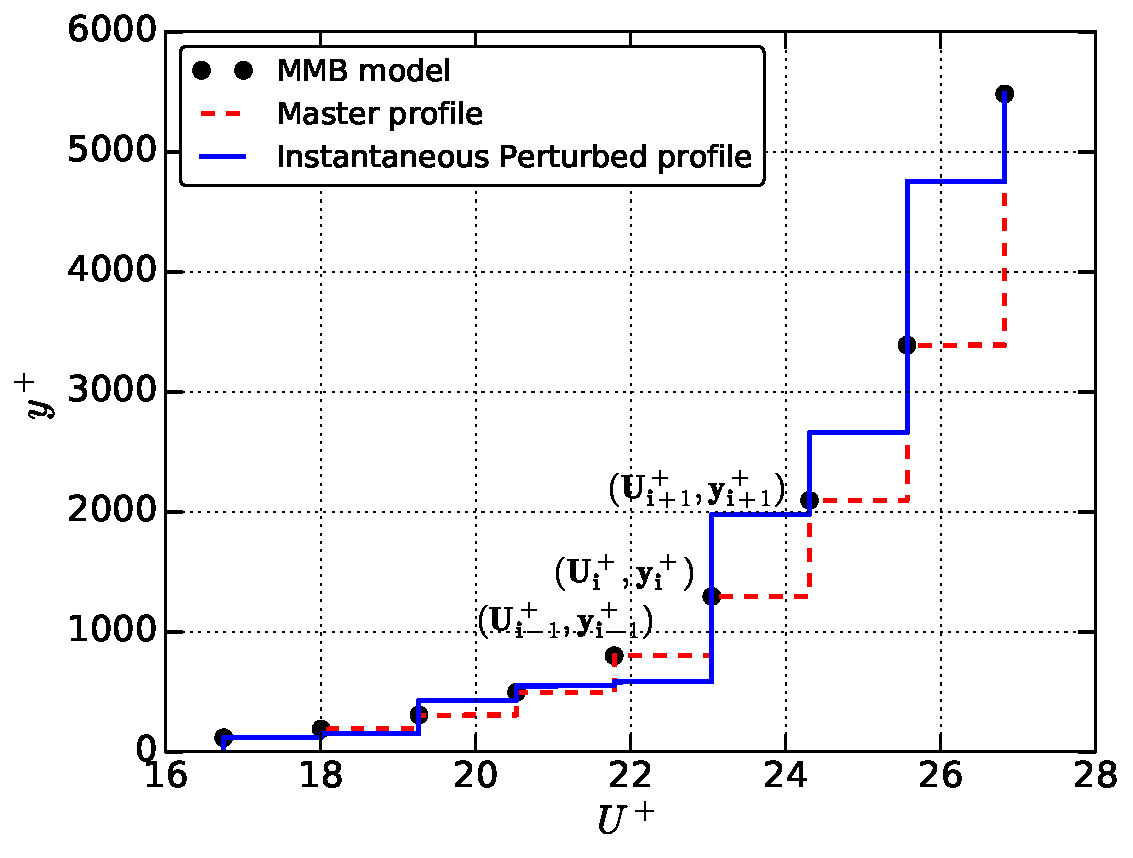
\includegraphics[scale=0.45]{figures/Master_step_profilev2}
\caption{\label{fig:master_profile} Mean step velocity master profile (red dashed lines) overlapped with an instantaneous perturbed velocity profile (blue solid line) and the original data points (filled black circles) computed by Eqs.~\eqref{eq:upvel} and~\eqref{eq:yppos}. $\delta^+=5200$ and $U^+_{\infty}=26.5$ are from channel DNS~\citep{leemoser2015}.}
\end{figure} 


Fig.~\ref{fig:master_profile} illustrates the mean step master velocity profile with a grid of $5481$ linearly spaced positions in the wall normal direction, each one with an associated streamwise velocity. The black dots are the velocities and positions of the vortical fissures computed using~\eqref{eq:upvel} and~\eqref{eq:yppos} respectively. Then the zones of uniform momentum are created by allocating the velocity of the current vortical fissure to the grid points between the previous $y_{i-1}$ and the current vortical fissure $y_i$. This velocity remains characteristic for each vortical fissure, thus we wave $N-1$ uniform momentum zones, where $N$ is number of the vortical fissures. Note that at higher $\delta^+$ the number of UMZs increases.
Next, instantaneous velocity profiles are created by the repositioning of the vortical structures through the wall normal direction. This is accomplished by add a perturbation of the actual height $\Delta h^+_i=y^+_i-y^+_{i-1}$ of the UMZ to the current position of the vortical fissure $y^+_i$, i.e, 
\begin{equation}\label{eq:ypert}
y^+_{new}=y^+_i\pm \Delta h^+_i*PERT.
\end{equation}

PERT stands for any statistical distribution used into perturb the height of the UMZ (e.g. Gaussian, uniform exponential, beta, etc). 
Here we remark that just the position of the vortical fissures are being perturbed though the velocities remains attached to each vortical fissure. Thus zones of higher momentum can reside closer to the wall if the upper vortical fissures move enough downward in the boundary layer. Once the new positions have been computed, we proceed to fill the grid points similarly to the master profile. Fig.~\ref{fig:master_profile} shows how most of the vorticals fissure have moved upward excepting the second and fifth that have moved downward respect to their original positions (blue solid line).  Fig.~\ref{fig:mul_profiles} shows five instantaneous velocity step profiles,  it can be seen how the upper vortical fissures resides now in the vicinity of the wall and some lower vortical fissures have moved to intermediate positions, this mechanism allow us to create zones of negative vorticity since the  uniform momentum zones are not increasing monotonically. 

\begin{figure}[tbh]
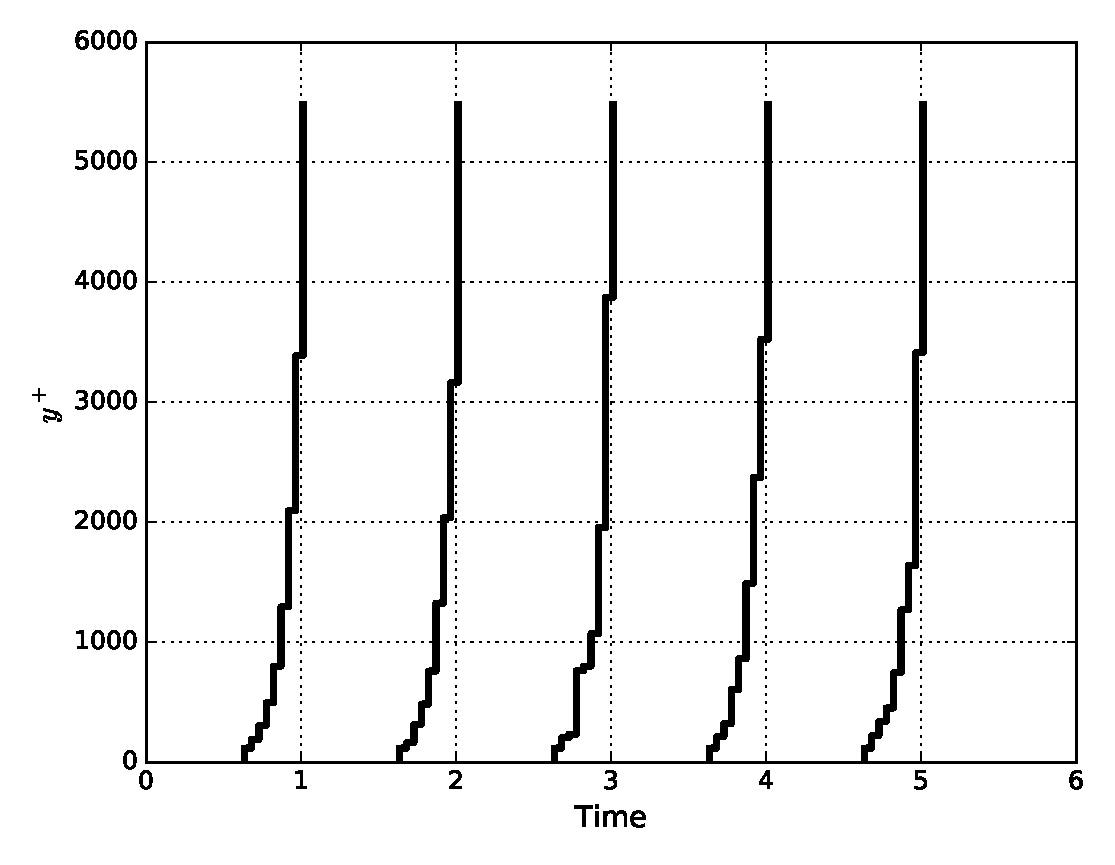
\includegraphics[scale=0.45]{figures/multiple_instantaneous_vprof}
\caption{\label{fig:mul_profiles} Multiple instantaneous velocity profiles with a gaussian perturbation of mean $\mu=0$ and standard deviation $\sigma=0.4$.}
\end{figure}

The multiple instantaneous step velocity profiles are considered independent events since they are the result of the statistical perturbation in the wall normal positions of the master profile.
\section{Mean turbulence statistics analysis}
For the purpose of validate the toy model, the high order moments such as the mean, variance, skewness and kurtosis of the mean turbulent streamwise velocity profile were computed. As described in Sec.~\ref{sec:nm}, not only a Gaussian perturbation was used to randomize the positions of the vortical fissure but also an uniform distribution. These variations attempts to explore if there is a dependence between the perturbation distribution and the statistics of the toy model. Thus a strong agreement between the numerical results either for any perturbation and the experimental data could give us some insight about the statistical nature of this process in a real turbulent flow.
\subsection{Gaussian perturbation}
Multiple scenarios with different standard deviations were investigated for the Gaussian perturbation, however just two are presented here. They represent poor ($\sigma=0.4$) and good ($\sigma=1$) agreement with the experimental results~\cite{Vincenti2013,FLM}, both with $\mu=0$. First scenario considers that the random variation in the position of the vortical fissures ranges between $-120\%$ and $120\%$ of their current positions, where $3\sigma$ events are less likely to occur. Fig.~\ref{fig:mean_profile} is the turbulent mean velocity profile for $\sigma=0.4$. It can be appreciated regions of relative uniform velocity along with small velocity jumps located close to the unperturbed wall normal positions of the vortical fissures (see Fig.~\ref{fig:master_profile}). These oscillations are similar to the peak-locking phenomena in experimental data, and they are the result of  the velocity average of vortical fissures with identical velocities in the same wall normal positions. Also note that an uniform momentum zone arise from $y^+=0$ to $y^+=118$, these are the velocity boundary conditions imposed in the first position of the vortical fissure which are held fixed. Despite of these discrepancies, the mean velocity profile shows an acceptable agreement with the shape of the experimental data.\\
\begin{figure}[b]
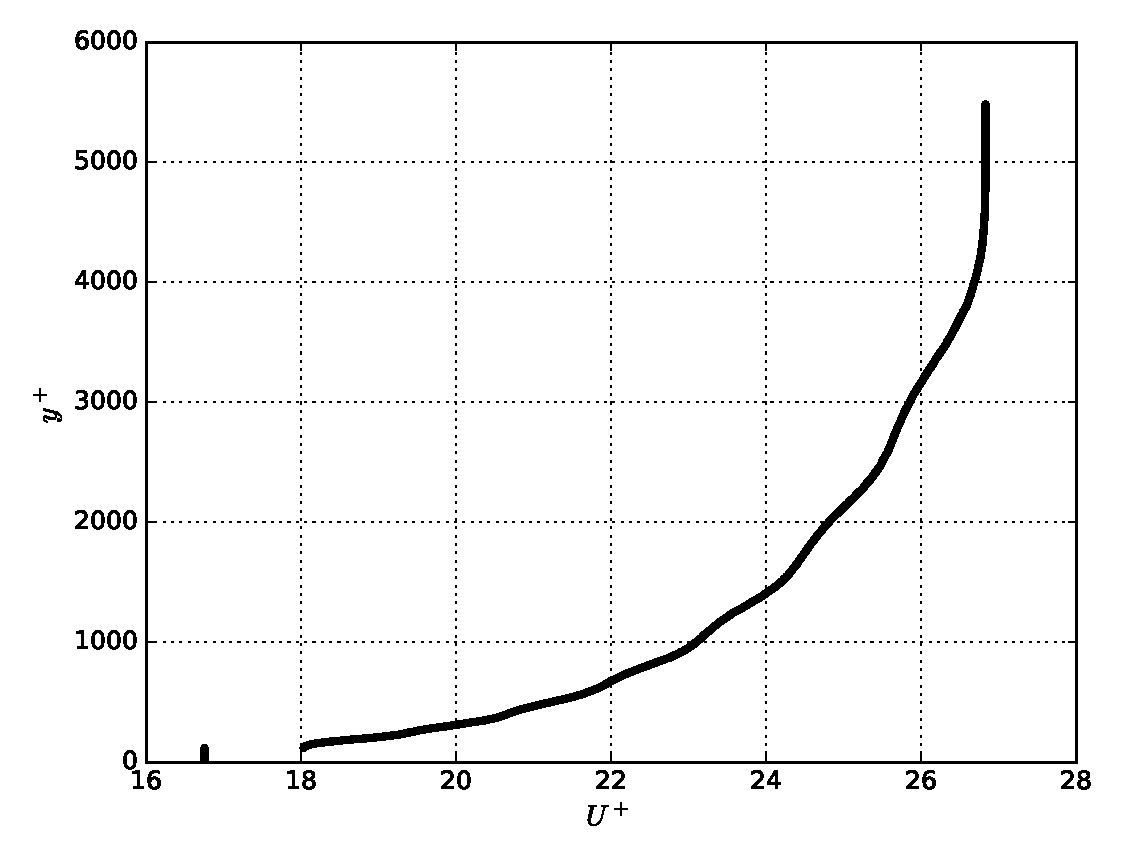
\includegraphics[scale=0.45]{figures/Master_averaged_step_profile_5000_assembles}
\caption{\label{fig:mean_profile} Mean stream-wise velocity profile for 5000 independent realizations with a Gaussian perturbation of $\mu=0$ and $\sigma=0.4$.}
\end{figure}

Fig.~\ref{fig:varigaus} shows the variance of the streamwise fluctuations for $5000$ independent realizations as a function of the wall normal position. Here the peak-locking phenomena is more evident and it could be associated to the use of pseudo-random number generators (PRNG). Since the Gaussian random numbers are not totally independent but they are computed through a deterministic algorithm, wall normal positions can be populated with the same vortical fissures several times~\cite{nm}. It is also remarkable that for this scenario crossing vortical fissures are rarely observed since the random perturbation does not exceed $130\%$ units of their current wall normal positions. 

\begin{figure}[tb]
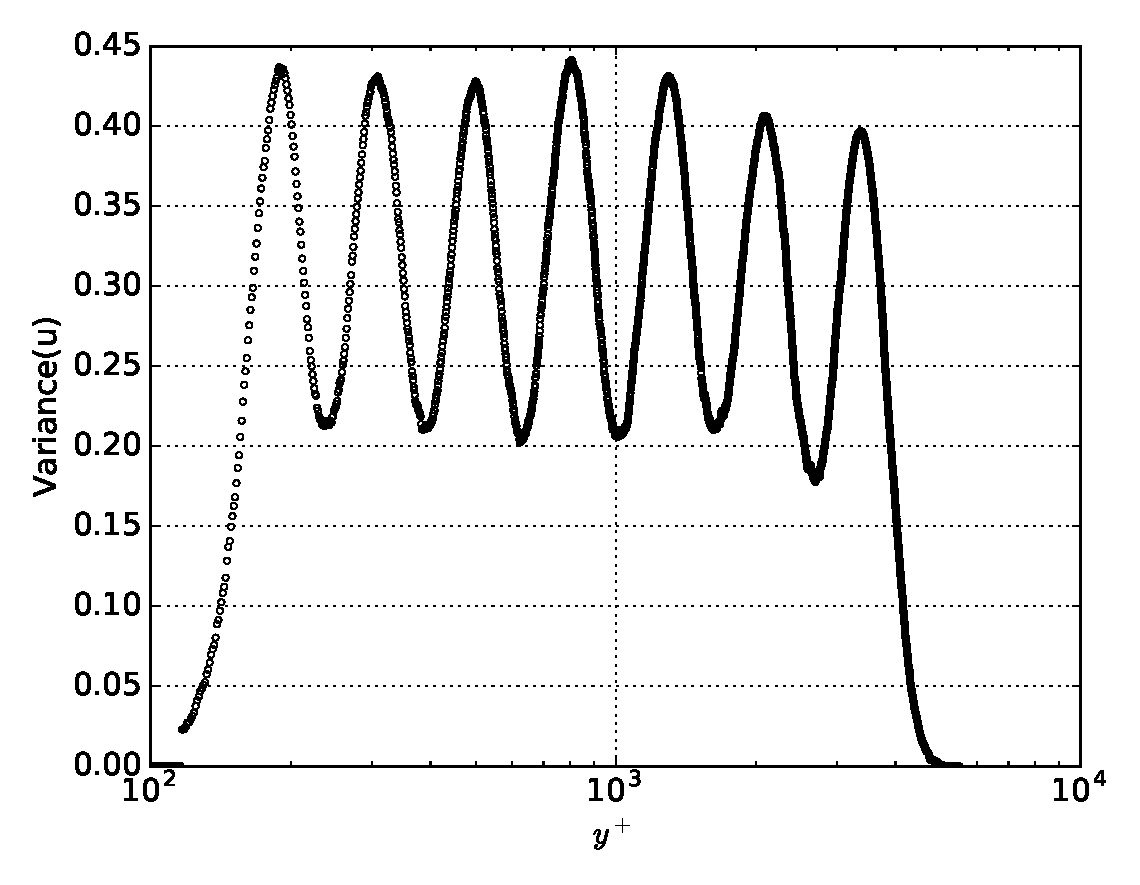
\includegraphics[scale=0.46]{figures/variance_5000_assembles}
\caption{\label{fig:varigaus} Stream-wise velocity variance for 5000 independent realizations with a Gaussian perturbation of $\mu=0$ and $\sigma=0.4$.}
\end{figure}
As is usual Fig.~\ref{fig:skewgaus} shows the skewness for the streamwise fluctuations as a function of the wall normal position on a semi-logarithmic axes plot. The graph shows the correct trend in the lower and the upper edge of the inertial region (Layer III table), i.e. it is maximum in the proximity of the wall and then it reaches its maximum negative value close to the boundary layer thickness $y^+=\delta^+$. However through the inertial region the skewness oscillates with an small amplitude $\pm 1$ around the value for a Gaussian distribution, in contrast with the experimental data that shows a plateau tendency right below of the Gaussian trend. The abrupt variations in the skewness can be also a side effect of peak-locking. Unlike the skewness, the oscillations for the stream-wise velocity kurtosis (Fig.~\ref{fig:kurt}) have a higher amplitude trough the inertial region where the experimental data exhibit an uniform subgaussian trend. This behaviour does not reproduce properly the turbulence statistics and thus we explore higher values of $\sigma$ in the Gaussian perturbation.

\begin{figure}[tb]
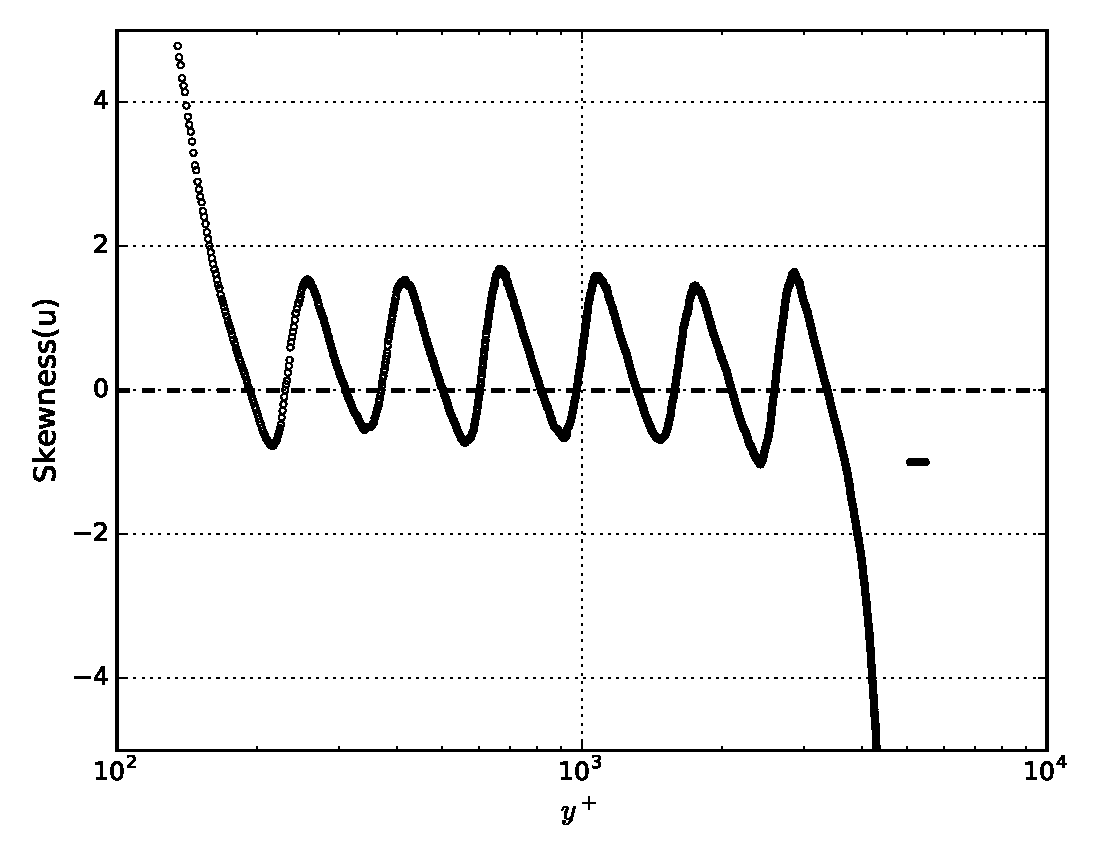
\includegraphics[scale=0.46]{figures/skewness_5000_assembles}
\caption{\label{fig:skewgaus} Skewness of streamwise velocity fluctuations for 5000 independent realizations with a Gaussian perturbation of $\mu=0$ and $\sigma=0.4$ (open circles). The skewness for a Gaussian distribution is plotted in dotted lines as reference.}
\end{figure}
In the second scenario $\sigma=1$ is selected in order to achieve a more homogeneous velocity distribution. This perturbation creates a random vertical motion of the vortical fissures between $-300\%$ and $300\%$ of their respective step height (see Sec.~\ref{sec:nm}). Consequently the vortical fissures in the upper edge of the inertial region can cross and reside close to the wall. The opposite is also true for vortical motions that lie in the onset of the inertial region. Fig.~\ref{fig:mp_gau100} shows a smoother profile compared with $\sigma=0.4$ where peak-locking effect was still present. This mean velocity profile exhibits a good agreement for $\delta^+=5200$ respect to the experimental data. 
\begin{figure}[tb]
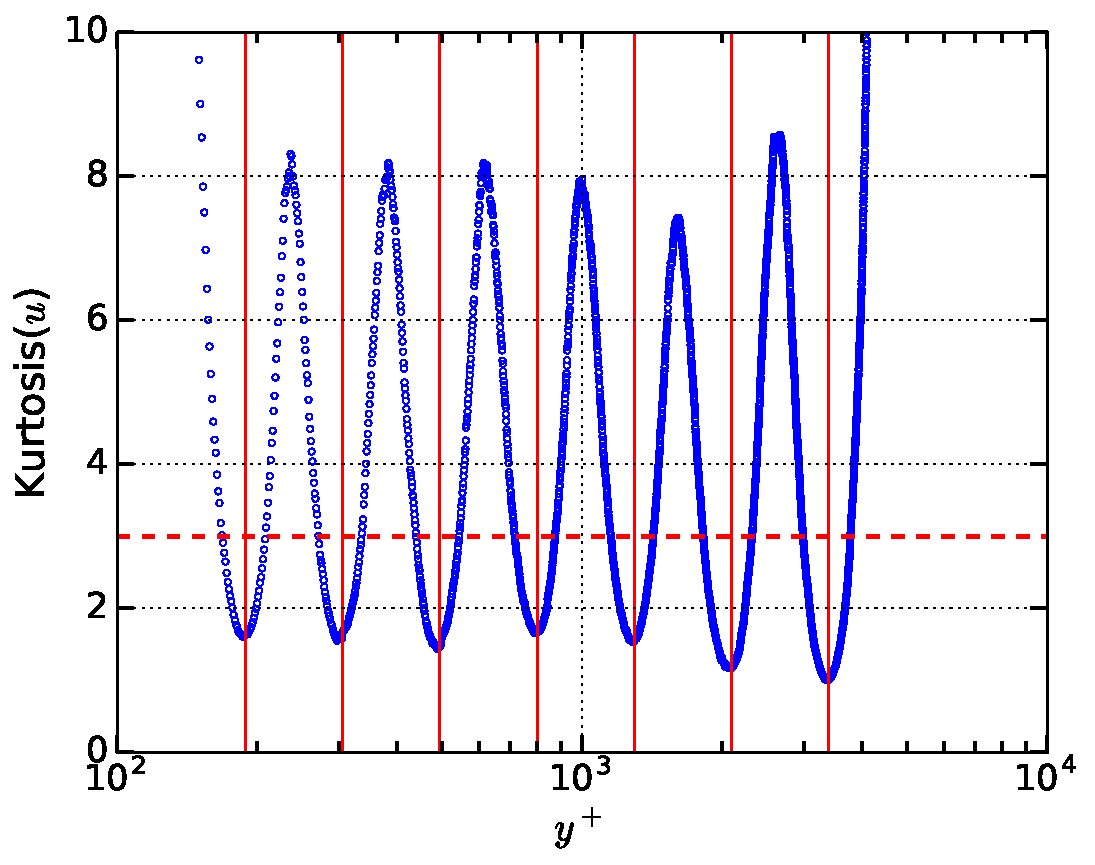
\includegraphics[scale=0.46]{figures/kurtosis_5000_assembles}
\caption{\label{fig:kurt} Kurtosis of streamwise velocity fluctuations for 5000 independent realizations with a Gaussian perturbation of $\mu=0$ and $\sigma=0.4$ (open circles). The kurtosis for a Gaussian distribution is plotted in dotted lines as reference.}
\end{figure}
In addition to the mean, the second, third and fourth order moments are also computed for this scenario. Fig.~\ref{fig:varigaus100} reveals some of the main properties of the stream-wise velocity variance for turbulent flows.  These are the variance is zero in the vicinity of the wall with its maximum value in the onset of the logarithmic region and then decreases almost logarithmically toward the boundary layer edge $y^+=\delta^+$. 
\begin{figure}[tb]
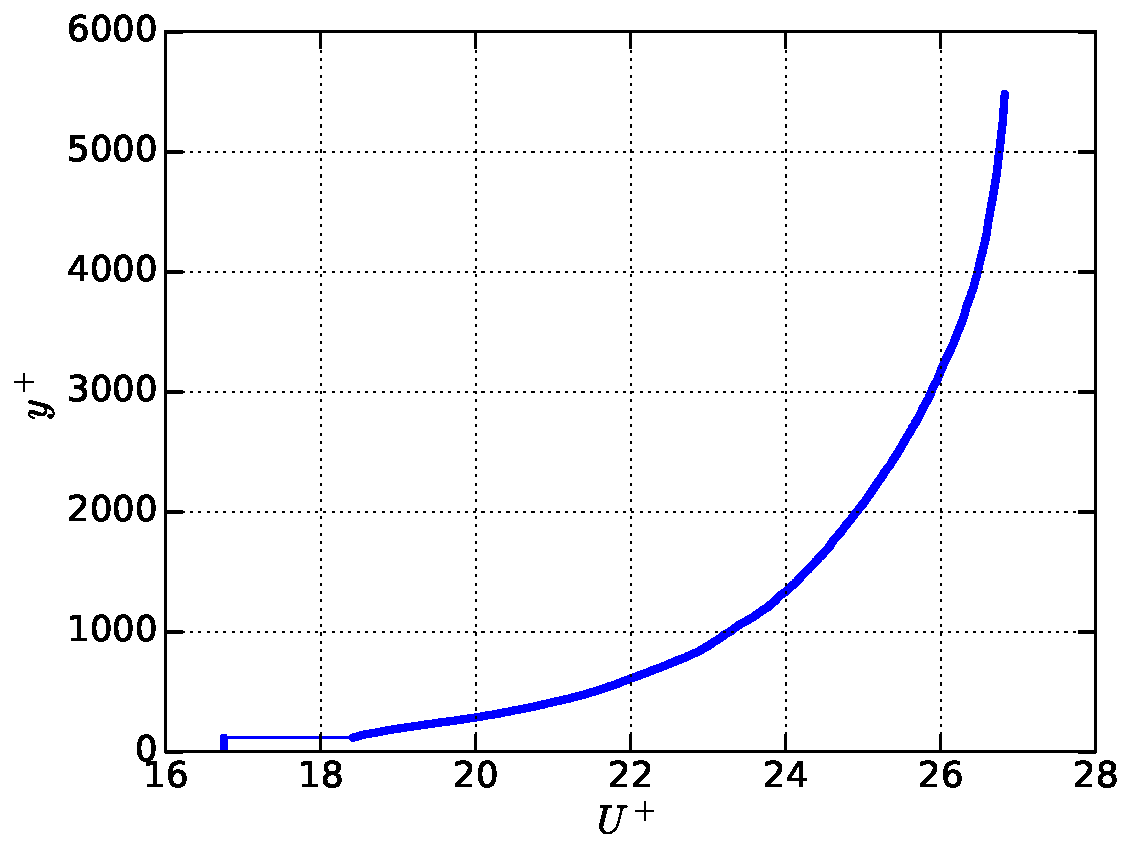
\includegraphics[scale=0.45]{figures/Master_averaged_step_profile_5000_assembles_gauss100}
\caption{\label{fig:mp_gau100} Mean turbulent stream-wise velocity profile for 5000 independent realizations with a Gaussian perturbation of $\mu=0$ and $\sigma=1$.}
\end{figure}
Although the variance is not totally smooth, it is a good improvement over the variance for the first scenario. Also note there is not evidence of peak-locking effect like can be visualized in the third and fourth moments (Figs.~\ref{fig:skewgaus100} and~\ref{fig:kurtgaus100}). 
\begin{figure}[b]
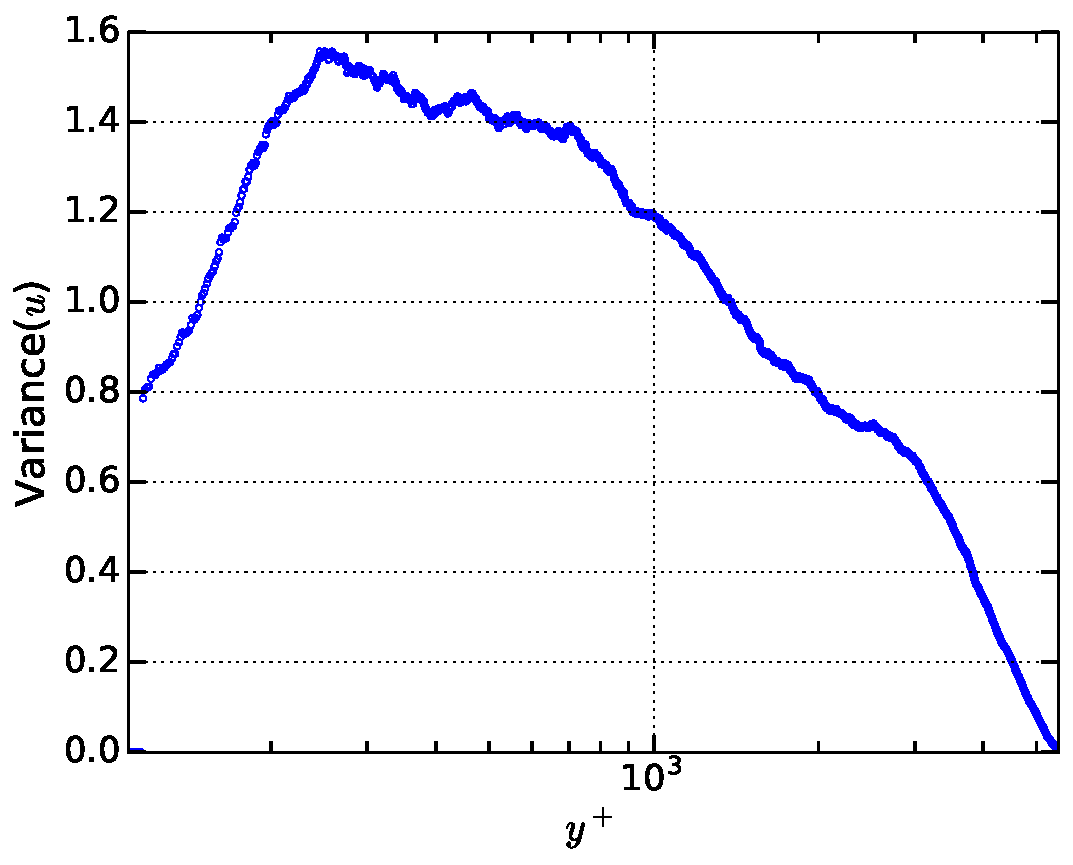
\includegraphics[scale=0.46]{figures/variance_5000_assembles_gauss100}
\caption{\label{fig:varigaus100} Stream-wise velocity variance for 5000 independent realizations with a Gaussian perturbation of $\mu=0$ and $\sigma=1$.}
\end{figure}
Fig.~\ref{fig:skewgaus100} shows the skewness for $\sigma=1$, it can be appreciated how the skewness has its maximum positive value close to the wall and then when it is approaching to the log region exhibits a subgaussian trend that rapidly decays to its maximum negative peak at the end of the logarithmic region. Unlike the experimental results, the boundaries of the skewness in the toy model still do not show the adequate trend. This is caused mainly because the first and last step vortical positions in the model are not being perturbed. Further investigation is necessary to establish the proper boundary conditions in order to improve the agreement near to the wall and away from it in the boundary layer for the turbulent statistics.
\begin{figure}[tb]
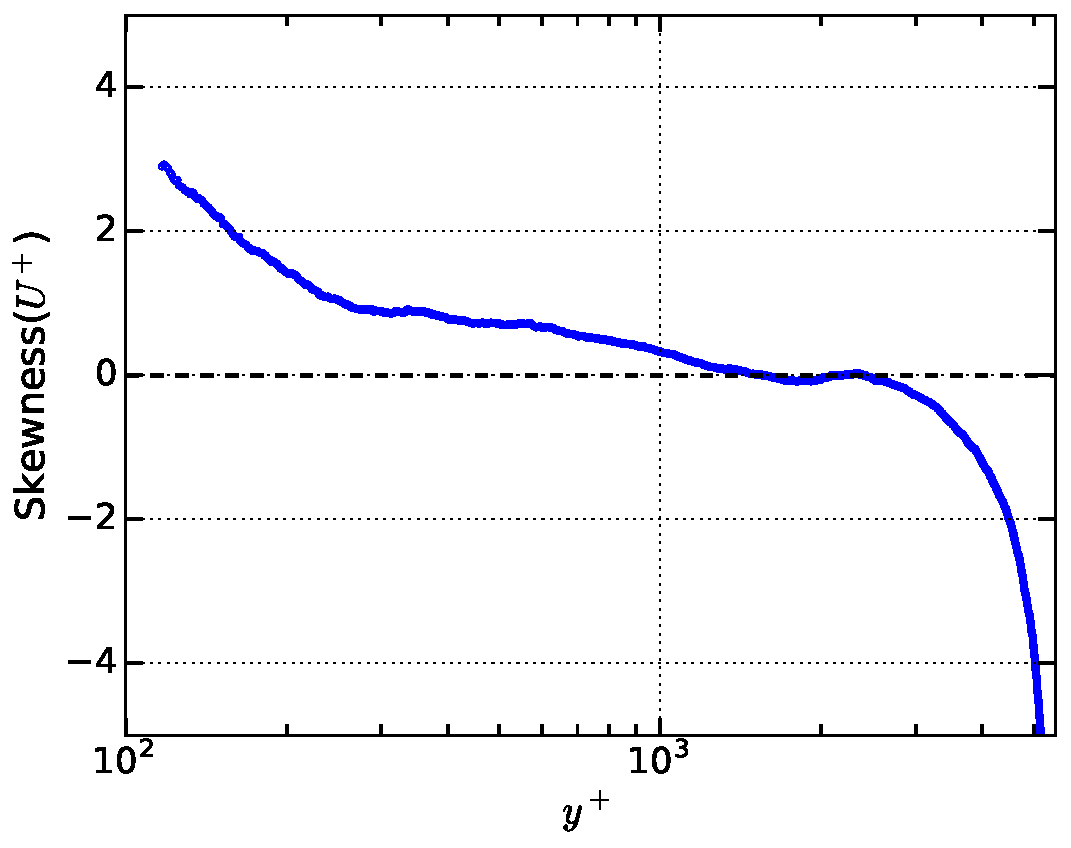
\includegraphics[scale=0.46]{figures/skewness_5000_assembles_gauss100}
\caption{\label{fig:skewgaus100} Skewness of streamwise velocity fluctuations for 5000 independent realizations with a Gaussian perturbation of $\mu=0$ and $\sigma=1$ (open circles). The skewness for a Gaussian distribution is plotted in dotted lines as reference.}
\end{figure}
Observation of Fig.~\ref{fig:kurtgaus100} evidences a similar pattern for the streamwise kurtosis, where the behaviour of the trend in the boundaries does not reproduce the experimental results faithfully. Despite of these discrepancies the kurtosis is very well behaved in the inertial region where it exhibits a subgaussian trend just as the real data do. Experimentally it is expected that the kurtosis reach its maximum value at $y^+=\delta^+$ and then decay in the free-stream region outside to the boundary layer. This is not observed in our results due to the boundary conditions explained previously. However a new distribution to perturb the position of the vortical fissures is attempted, one whose edges decays smoother than the gaussian distribution, thus a dependence on the perturbation distribution can be discarded.
\begin{figure}[tb] 
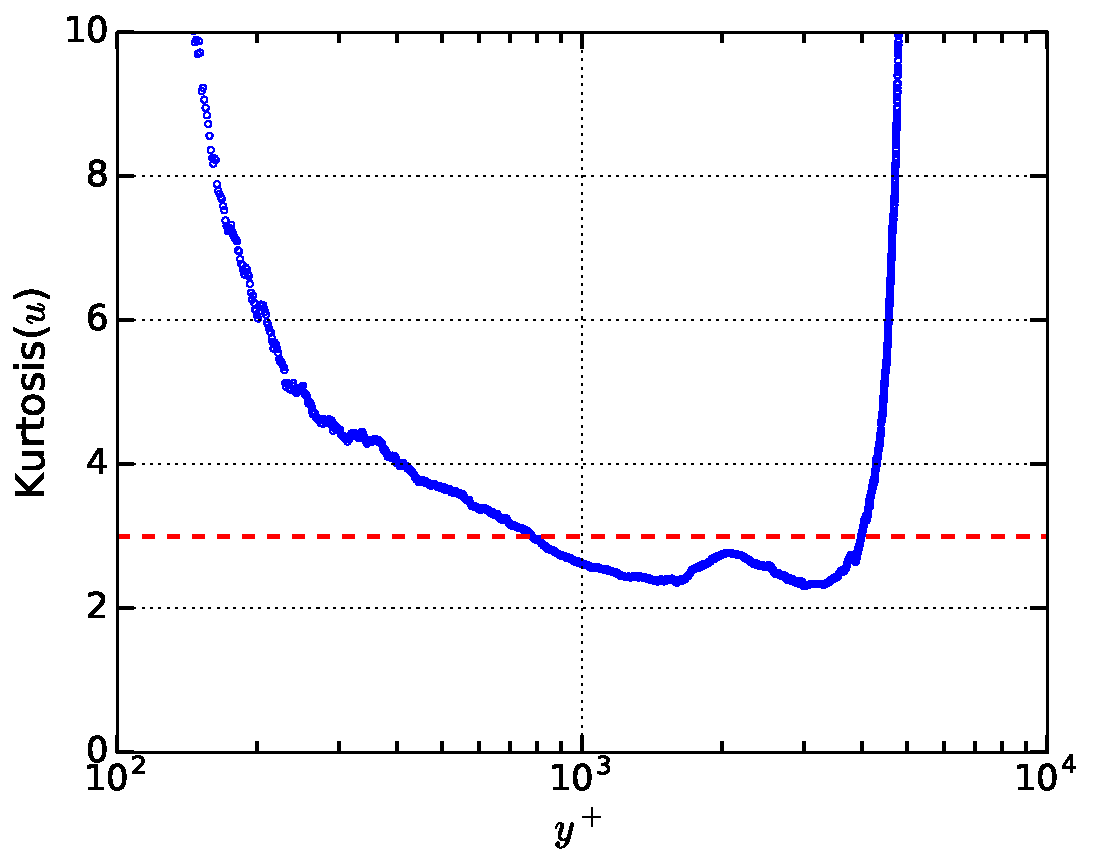
\includegraphics[scale=0.46]{figures/kurtosis_5000_assembles_gauss100}
\caption{\label{fig:kurtgaus100} Kurtosis of streamwise velocity fluctuations for 5000 independent realizations with a Gaussian perturbation of $\mu=0$ and $\sigma=1$ (open circles). The kurtosis for a Gaussian distribution is plotted in dotted lines as a reference.}
\end{figure}
Next section describe the numerical results of the turbulence statistics using an uniform distribution.
\subsection{Uniform distribution}
Previous section suggest that the vortical fissure crossing enhances the creation of a more homogeneous velocity distribution in the boundary layer, therefore an uniform distribution between $-130\%$ and $130\%$ of the height of the step has been selected. Fig.~\ref{fig:mp_un130}  shows the streamwise velocity profile for the uniform perturbation. In comparison with Fig~\ref{fig:mean_profile}, the jumps in the velocity profile seems to have a more straight slope. Since for an uniform distribution, all the vortical positions have the same probability to occur, regions of concentrated velocity such like in the gaussian distribution are not observed. Instead zones with an increasing uniform velocity are appreciated.   

\begin{figure}[tbh]
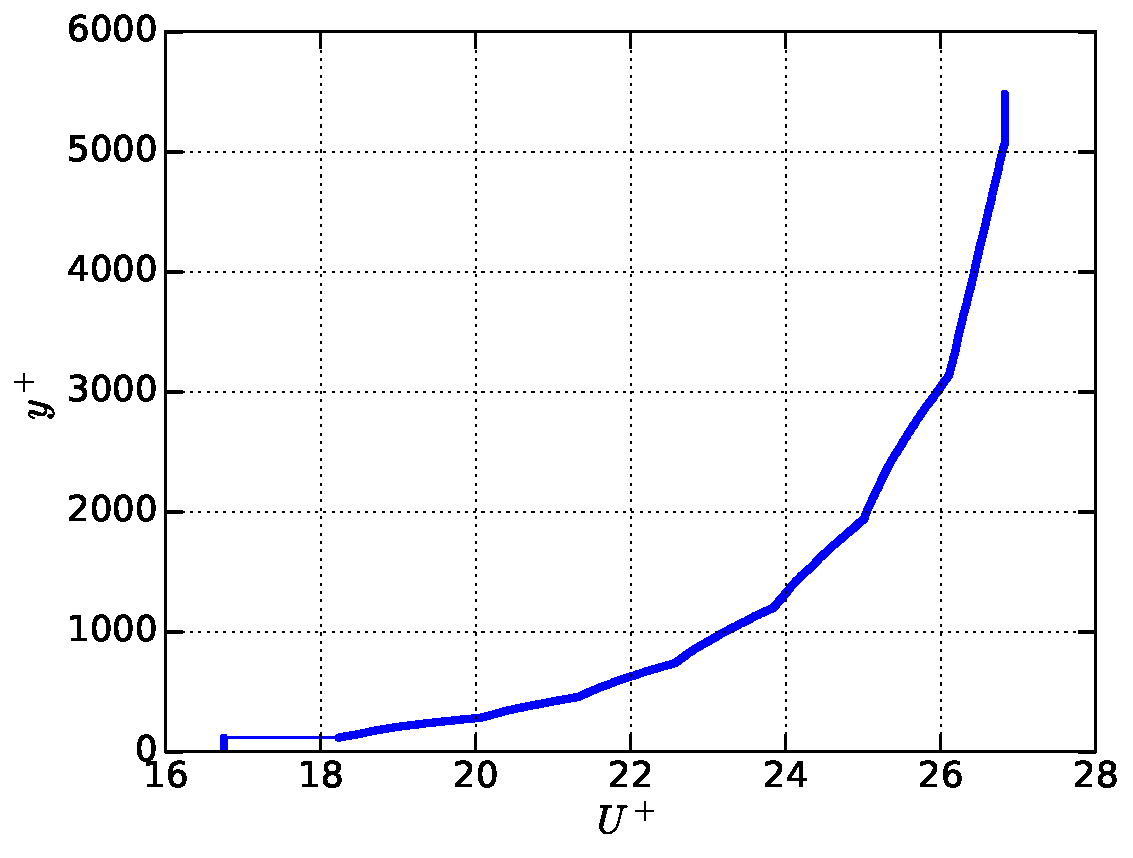
\includegraphics[scale=0.45]{figures/Master_averaged_step_profile_5000_assembles_un130}
\caption{\label{fig:mp_un130} Mean turbulent stream-wise velocity profile for 5000 independent realizations with an uniform perturbation of $\pm 130\%$.}
\end{figure}

This effect can be appreciated more clearly in the stream-wise velocity variance (Fig.~\ref{fig:varun130}), where the variance oscillates around the positions of the vortical fissures in the master profile. These oscillations are characterized by having a smaller amplitude ($\sim 0.2$ units) compared with the Gaussian perturbation for $\sigma=0.4$ (Fig.~\ref{fig:varigaus}). Despite of the oscillations, the main features of the turbulence variance are conserved. For instance it has a peak in the proximity of the wall and then a pronounced negative slope in the inertial region up to reach zero in the upper edge of the inertial region.\\
\begin{figure}[tbh]
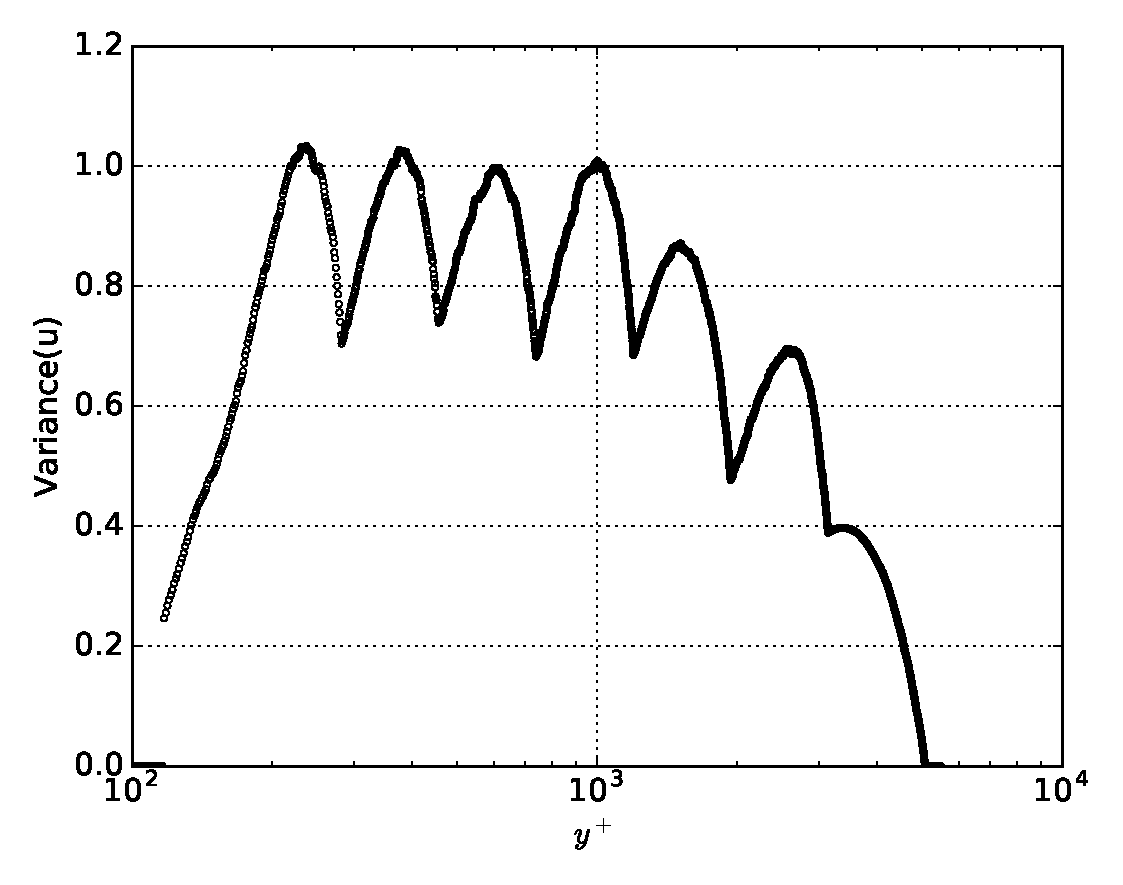
\includegraphics[scale=0.46]{figures/variance_5000_assembles_un130}
\caption{\label{fig:varun130} Variance of streamwise velocity fluctuations for 5000 independent realizations with an uniform perturbation of $\pm \%130$.}
\end{figure}     
The rapid variations still persist in the higher order moments, however their amplitude are smaller compared with the gaussian distribution for $\sigma=0.4$. Fig.~\ref{fig:skewun130} shows the skewness of the streamwise velocity for an uniform distribution. A strong agreement in the main features between the numerical simulation and the experimental skewness is observed, in brief the skewness follows a pseudo-Gaussian trend in the inertial region , then it increases up to reach its maximum negative value in the upper limit of the boundary layer $y^+=\delta^+$ to after finally decay to zero in the free-stream region.
\begin{figure}[tb]
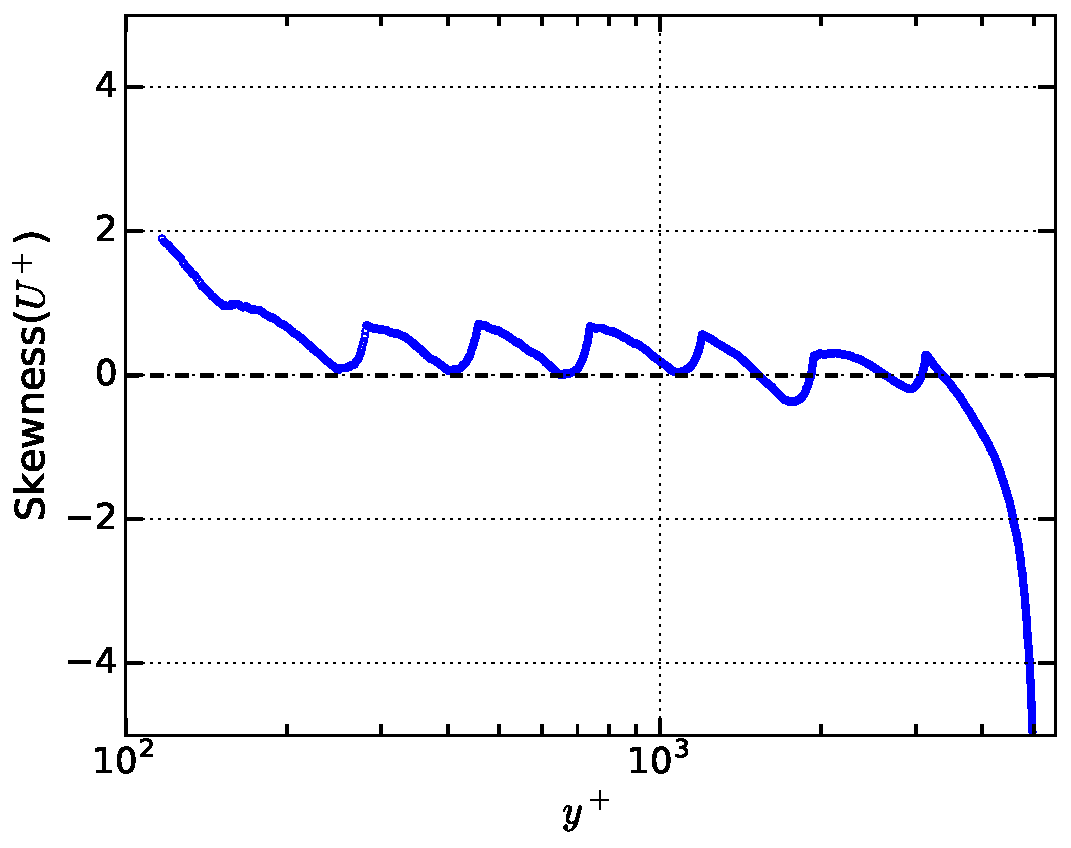
\includegraphics[scale=0.46]{figures/skewness_5000_assembles_un130}
\caption{\label{fig:skewun130} Skewness of streamwise velocity fluctuations for 5000 independent realizations with an uniform perturbation of $\pm 130\%$ (open circles). The skewness for a Gaussian distribution is plotted in dotted lines as a reference.}
\end{figure}
Fourth order moment is illustrated in Fig.~\ref{fig:kurtun130}, the trend is in complete concordance with the experimental data if the small oscillations are neglected. Further exploration is needed to improve the right behaviour in the upper and lower limits of the inertial region.
\begin{figure}[tbh] 
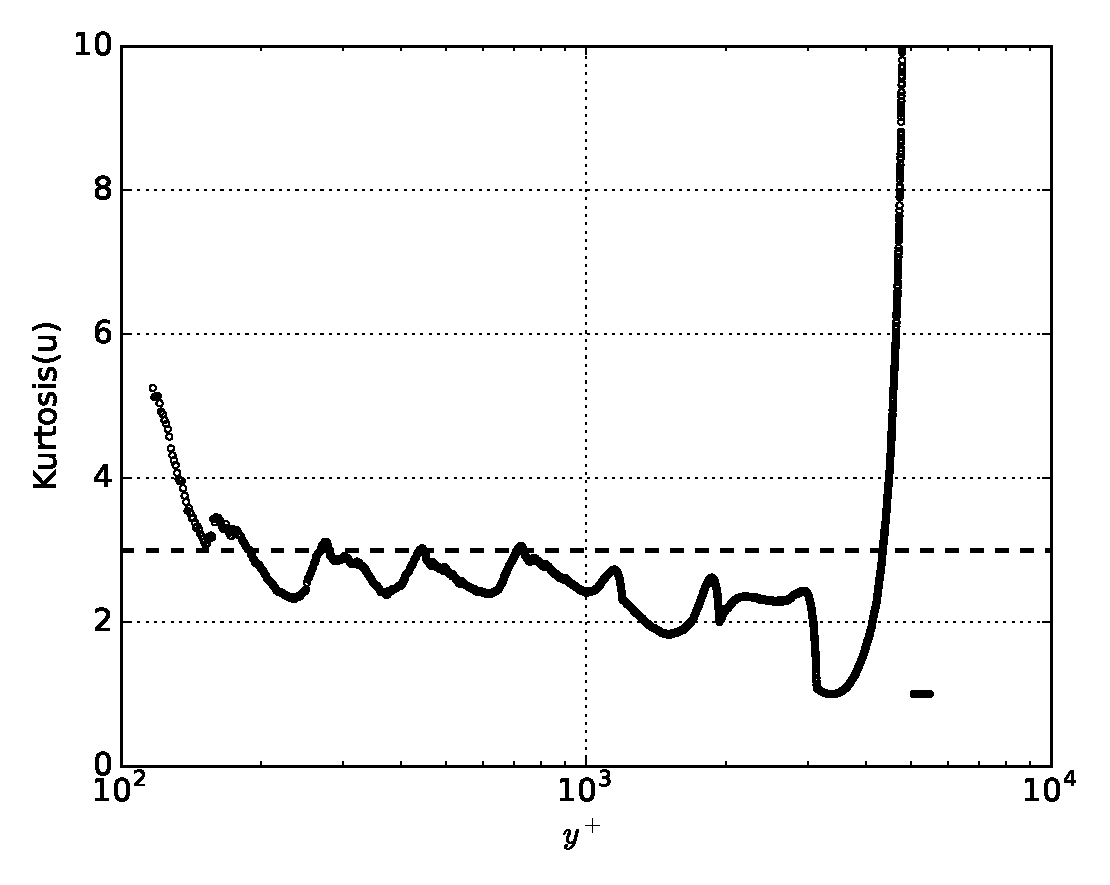
\includegraphics[scale=0.46]{figures/kurtosis_5000_assembles_un130}
\caption{\label{fig:kurtun130} Kurtosis of streamwise velocity fluctuations for 5000 independent realizations with an uniform perturbation of $\pm 130\%$ (open circles). The kurtosis for a Gaussian distribution is plotted in dotted lines as a reference.} 
\end{figure}

\section{Conclussions}
Several statistical distribution were used to explore the appropriate behaviour of the higher order moments. It was found that just the Gaussian and the uniform distribution reproduce the right structure of the turbulent boundary layer. The results also reveal that in order to have similar qualitative statistics to the experimental data, the vortical fissures need to cross through the boundary layer. Hence that the percentages of perturbation for the Gaussian and uniform perturbation must be at least $100\%$ and $130\%$ respectively. Higher percentages were also explored but there were not either qualitative or quantitative improvements in the statistics. Further observation of the mean streamwise-velocity profile allows to infer that an inertial region in the turbulent boundary layer exist between $y^+=10^3$ trough $y^+=3\times 10^3$ approximately.  These results support the main hypothesis of this paper, namely the boundary layer structure is the result of the long-time averaged of instantaneous velocity profiles with different distributions of UMZs. 

%\nocite{*}
\bibliography{Aps_template2}% Produces the bibliography via BibTeX.
\end{document}
